\section{General approach}
\label{sec:exploratory-study:methodology}

\subsection{Data collection}
\label{sec:exploratory-study:methodology:case-software-tools}

A meta-analysis\index{Meta-analysis} involving a total of 12 software applications
was systematically conducted to facilitate the compilation of a comprehensive
and inclusive set of principles. The set of tools comprised six
\gls{dl} software applications and six non-\gls{dl}
software applications. The selection of the six \gls{dl} software
was done on the basis of popularity as depicted on
OpenDOAR\footnote{\url{http://www.opendoar.org}}\index{OpenDOAR}. Table~\ref{tab:exploratory-study:methodology:case-software} outlines the 12 candidate tools that were considered.

The relevant software attributes that may have influenced the design decisions
of the applications were then identified. The pairwise comparisons method,
outlined in Section~\ref{sec:exploratory-study:research-methods:ahp:pairwise} was then used as
the constant comparison method during the data analysis stage. The data
analysis stage is discussed in more detail in Section~\ref{sec:exploratory-study:methodology:data-analysis}

% Software applications table

\tablespacing
%%%%%\begin{longtable}{p{0.25\linewidth} p{0.25\linewidth} p{0.4\linewidth}}
\begin{longtable}{
>{\arraybackslash}p{0.22\linewidth}|
>{\arraybackslash}p{0.20\linewidth}|
>{\arraybackslash}p{0.48\linewidth}}

\caption{Software applications used for pairwise comparisons}
\label{tab:exploratory-study:methodology:case-software} \\

 %%%%%\toprule
 %%%%%\hline
 \textbf{Application} & \textbf{Category} & \textbf{Description}\\
 %%%%%\midrule
 \cline{1-3}
 \endfirsthead

 \caption[]{(continued)}\\
 %%%%%\toprule
 %%%%%\hline
 \textbf{Application} & \textbf{Category} & \textbf{Description}\\
 %%%%%\midrule
 \cline{1-3}
 \endhead

 % Page footer
 %%%%%\midrule
 %%%%%\hline
 \multicolumn{3}{r}{(Continued on next page)} \\
 \endfoot

 % Last page footer
 %%%%%\bottomrule
 \endlastfoot

 \textbf{DSpace\footnote{\url{http://www.dspace.org}}}&
 {DL software}&
 {A general digital asset management software}\\

 \cline{1-3}
 %\cmidrule[0.1pt](l{0.5em}r{0.5em}){1-3}

 \textbf{EPrints\footnote{\url{http://www.eprints.org}}}&
 {DL software}&
 {A general digital repository software package}\\

 \cline{1-3}
 %\cmidrule[0.1pt](l{0.5em}r{0.5em}){1-3}

 \textbf{ETD-db\footnote{\url{http://scholar.lib.vt.edu/ETD-db}}}&
 {DL software}&
 {An electronic thesis and dissertation software package}\\

 \cline{1-3}
 %\cmidrule[0.1pt](l{0.5em}r{0.5em}){1-3}

 \textbf{FedoraCommons\footnote{\url{http://fedora-commons.org}}}&
 {DL software}&
 {A general digital object repository framework}\\

 \cline{1-3}
 %\cmidrule[0.1pt](l{0.5em}r{0.5em}){1-3}

 \textbf{Greenstone\footnote{\url{http://www.greenstone.org}}}&
 {DL software}&
 {A general digital collection management software}\\

 \cline{1-3}
 %\cmidrule[0.1pt](l{0.5em}r{0.5em}){1-3}

 \textbf{CDS Invenio\footnote{\url{http://invenio-software.org}}}&
 {DL Software}&
 {A general document repository software package}\\

 \cline{1-3}
 %%%%%\cmidrule[0.1pt](l{0.5em}r{0.5em}){1-3}
 %%%%%\cline{1-3}

 \textbf{Facebook\footnote{\url{http://www.facebook.com}}}&
 {Non DL software}&
 {A free social network portal/Website}\\

 \cline{1-3}
 %\cmidrule[0.1pt](l{0.5em}r{0.5em}){1-3}

 \textbf{Gmail\footnote{\url{https://mail.google.com}}}&
 {Non DL software}&
 {A free email messaging hosted-service platform}\\

 \cline{1-3}
 %\cmidrule[0.1pt](l{0.5em}r{0.5em}){1-3}

 \textbf{MixIt\footnote{\url{http://www.mixit.com}}}&
 {Non DL software}&
 {A free instant messaging Web application}\\

 \cline{1-3}
 %\cmidrule[0.1pt](l{0.5em}r{0.5em}){1-3}

 \textbf{Moodle\footnote{\url{http://moodle.org}}}&
 {Non DL software}&
 {A free e-learning management platform}\\

 \cline{1-3}
 %\cmidrule[0.1pt](l{0.5em}r{0.5em}){1-3}

 \textbf{Ushahidi\footnote{\url{http://www.ushahidi.com}}}&
 {Non DL software}&
 {An information collection and visualisation platform}\\

 \cline{1-3}
 %\cmidrule[0.1pt](l{0.5em}r{0.5em}){1-3}

 \textbf{WordPress\footnote{\url{http://wordpress.org}}}&
 {Non DL software}&
 {A standalone blogging software package}\\

 \end{longtable}

\bodyspacing

\subsection{Data analysis}
\label{sec:exploratory-study:methodology:data-analysis}

The set of all possible software attributes that can potentially influence
design decisions of software applications were identified and arranged based on
whether they were specific to the two sets of software applications---Digital
Library software and non-\gls{dl} software---or both sets. Table~\ref{tab:exploratory-study:methodology:software-attributes} shows the
software attributes, that were considered,  as pertains to whether they affect
\gls{dl} software, non-\gls{dl} software, or both.

\tablespacing
%%%%%\begin{longtable}{p{0.45\linewidth} p{0.15\linewidth} p{0.15\linewidth}
%%%%%p{0.15\linewidth}}
\begin{longtable}{
>{\arraybackslash}p{0.35\linewidth}|
>{\centering\arraybackslash}p{0.15\linewidth}|
>{\centering\arraybackslash}p{0.15\linewidth}|
>{\centering\arraybackslash}p{0.15\linewidth}}

\caption{Software attributes considered in pairwise comparisons}
\label{tab:exploratory-study:methodology:software-attributes} \\

 %%%%%\toprule
 %%%%%\hline
 %%%%%\textbf{} & 
 %%%%%\multicolumn{3}{c}{\textbf{Software Category}}\\
 %%%%%\midrule
 %%%%%\cline{2-4}
 \textbf{} &
 \textbf{DL} &
 \textbf{Non-DL} &
 \textbf{Both} \\
 %%%%%\midrule
 \cline{1-4}
 \endfirsthead

 \caption[]{(continued)}\\
 %%%%%\toprule
 %%%%%\hline
 %%%%%\textbf{} & 
 %%%%%\multicolumn{3}{c}{\textbf{Software Category}}\\
 %%%%%\midrule
 %%%%%\cline{2-4}
 \textbf{} &
 \textbf{DL} &
 \textbf{Non-DL} &
 \textbf{Both} \\
 %%%%%\midrule
 \cline{1-4}
 \endhead

 % Page footer
 %%%%%\midrule
 %%%%%\hline
 \multicolumn{4}{r}{(Continued on next page)} \\
 \endfoot

 % Last page footer
 %%%%%\bottomrule
 \endlastfoot

 \textbf{Digital content}&
 {X}&
 {}&
 {}\\

 \cline{1-4}
 %\cmidrule[0.1pt](l{0.5em}r{0.5em}){1-3}

 \textbf{Media types}&
 {X}&
 {}&
 {}\\

 \cline{1-4}
 %\cmidrule[0.1pt](l{0.5em}r{0.5em}){1-3}

 \textbf{Metadata objects}&
 {X}&
 {}&
 {}\\

 \cline{1-4}
 %\cmidrule[0.1pt](l{0.5em}r{0.5em}){1-3}

 \textbf{Data access}&
 {}&
 {}&
 {X}\\

 \cline{1-4}
 %\cmidrule[0.1pt](l{0.5em}r{0.5em}){1-3}

 \textbf{Information structure}&
 {X}&
 {}&
 {}\\

 \cline{1-4}
 %\cmidrule[0.1pt](l{0.5em}r{0.5em}){1-3}

 \textbf{Core language}&
 {}&
 {}&
 {X}\\

 \cline{1-4}
 %\cmidrule[0.1pt](l{0.5em}r{0.5em}){1-3}

 \textbf{Content delivery}&
 {}&
 {}&
 {X}\\

 \cline{1-4}
 %\cmidrule[0.1pt](l{0.5em}r{0.5em}){1-3}

 \textbf{Deployment platform}&
 {}&
 {}&
 {X}\\

 \cline{1-4}
 %\cmidrule[0.1pt](l{0.5em}r{0.5em}){1-3}

 \textbf{Software dependencies}&
 {}&
 {}&
 {X}\\

 \cline{1-4}
 %\cmidrule[0.1pt](l{0.5em}r{0.5em}){1-3}

 \textbf{Flexibility}&
 {}&
 {}&
 {X}\\

 \cline{1-4}
 %\cmidrule[0.1pt](l{0.5em}r{0.5em}){1-3}

 \textbf{Preservation strategy}&
 {X}&
 {}&
 {}\\

 \cline{1-4}
 %\cmidrule[0.1pt](l{0.5em}r{0.5em}){1-3}

 \textbf{Extensibility}&
 {}&
 {}&
 {X}\\

 \cline{1-4}
 %\cmidrule[0.1pt](l{0.5em}r{0.5em}){1-3}

 \textbf{Standardisation}&
 {}&
 {}&
 {X}\\

 \cline{1-4}
 %\cmidrule[0.1pt](l{0.5em}r{0.5em}){1-3}

 \textbf{Interoperability}&
 {}&
 {}&
 {X}\\

 \cline{1-4}
 %\cmidrule[0.1pt](l{0.5em}r{0.5em}){1-3}

 \textbf{Ease of installation}&
 {}&
 {}&
 {X}\\

 \cline{1-4}
 %\cmidrule[0.1pt](l{0.5em}r{0.5em}){1-3}

 \textbf{Objects accessibility}&
 {X}&
 {}&
 {}\\

 \cline{1-4}
 %\cmidrule[0.1pt](l{0.5em}r{0.5em}){1-3}

 \textbf{Objects naming scheme}&
 {X}&
 {}&
 {}\\

 \cline{1-4}
 %\cmidrule[0.1pt](l{0.5em}r{0.5em}){1-3}

 \textbf{Hosting}&
 {}&
 {}&
 {X}\\

 \cline{1-4}
 %\cmidrule[0.1pt](l{0.5em}r{0.5em}){1-3}
 
 \textbf{Scalability}&
 {}&
 {}&
 {X}\\

 \cline{1-4}
 %\cmidrule[0.1pt](l{0.5em}r{0.5em}){1-3}
 
 \textbf{Reliability}&
 {}&
 {}&
 {X}\\

 \cline{1-4}
 %\cmidrule[0.1pt](l{0.5em}r{0.5em}){1-3}
 
 \textbf{Usability}&
 {}&
 {}&
 {X}\\

 \cline{1-4}
 %\cmidrule[0.1pt](l{0.5em}r{0.5em}){1-3}

 \textbf{Mobile friendly}&
 {}&
 {}&
 {X}\\

 %%%%%\cline{1-4}
 %\cmidrule[0.1pt](l{0.5em}r{0.5em}){1-3}

 \end{longtable}

\bodyspacing

Open coding\index{Open Coding} \citep{Glaser1992} was used during the data analysis
process, and a head-to-head pairwise comparison was then performed on each of
the 12 applications against the other alternatives using the
pairwise comparisons method procedure described in Section~\ref{sec:exploratory-study:research-methods:ahp:pairwise}. All in all, a total
of 66 pairwise comparisons, derived using the equation in Section~\ref{sec:exploratory-study:research-methods:ahp:pairwise}, were conducted. 
%A template showing the detailed comparative attributes is shown in Table~\ref{tab:exploratory-study:methodology:digital-library-software} in Appendix~\ref{ch:appendex-a:exploratory-study}

The Memoing process\index{Memoing}, for each of the 66 comparisons, involved
identifying design choice for each software attribute and the possible
corresponding design rationale\index{Design Rationale}. All possible potential design decisions that
could be applicable to the design of simple and minimalistic architectures were
subsequently identified. Figure~\ref{fig:exploratory-study:general-approach:data-analysis:memoing-process}
shows an excerpt of the memoing process.

\begin{figure}
 \begin{center}
 \fbox{
 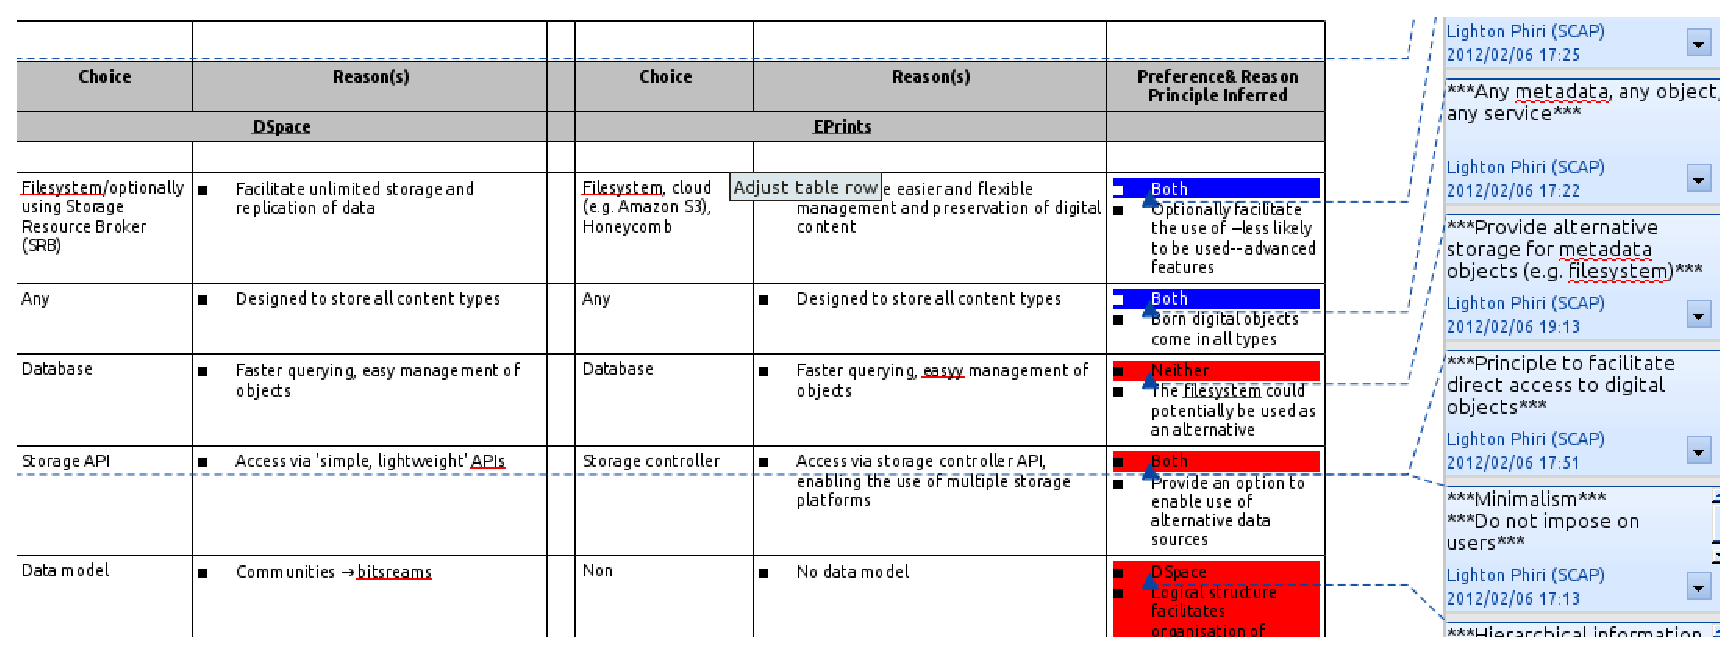
\includegraphics[width=0.95\textwidth]{%
chapter04/figures/grounded-theory-memoing.eps}
 }
 \caption[Screenshot showing an excerpt of the GT memoing process]{Screenshot showing an excerpt of the grounded theory memoing process}
 \label{fig:exploratory-study:general-approach:data-analysis:memoing-process}
 \end{center}
\end{figure}



% Defunct now---September 19, 2012
%
%Table showing attributes considered during general pairwise comparisons for all
%tools

%\tablespacing
%\begin{landscape}
%\begin{longtable}{p{0.25\linewidth} p{0.13\linewidth} p{0.13\linewidth}
p{0.13\linewidth} p{0.13\linewidth} p{0.13\linewidth}}

\caption{General Software Feature Pairwise Comparisons Matrix}
\label{tab:exploratory-study:methodology:general-software} \\

 \toprule
{} & \multicolumn{2}{c}{\textbf{Application 1}} &
\multicolumn{2}{c}{\textbf{Application 2}} & {}\\
 \midrule
\textbf{Attribute} & \textbf{Choice} & \textbf{Reason} & \textbf{Choice} &
\textbf{Reason} & \textbf{Comments}\\
 \midrule
 \endfirsthead

 \caption[]{(continued)}\\
 \toprule
{} & \multicolumn{2}{c}{\textbf{Application 1}} &
\multicolumn{2}{c}{\textbf{Application 2}} & {}\\
 \midrule
\textbf{Attribute} & \textbf{Choice} & \textbf{Reason} & \textbf{Choice} &
\textbf{Reason} & \textbf{Comments}\\
 \midrule
 \endhead

 % Page footer
 \midrule
 \multicolumn{6}{r}{(Continued on next page)} \\
 \endfoot

 % Last page footer
 \bottomrule
 \endlastfoot

 %\cmidrule[0.1pt](l{0.5em}r{0.5em}){1-6}

 {Hosting}&
 {\ldots}&
 {\ldots}&
 {\ldots}&
 {\ldots}&
 {\ldots}\\

 \cmidrule[0.1pt](l{0.5em}r{0.5em}){1-6}

 {Extensibility}&
 {\ldots}&
 {\ldots}&
 {\ldots}&
 {\ldots}&
 {\ldots}\\

 \cmidrule[0.1pt](l{0.5em}r{0.5em}){1-6}

 {Scalability}&
 {\ldots}&
 {\ldots}&
 {\ldots}&
 {\ldots}&
 {\ldots}\\

 \cmidrule[0.1pt](l{0.5em}r{0.5em}){1-6}

 {Reliability}&
 {\ldots}&
 {\ldots}&
 {\ldots}&
 {\ldots}&
 {\ldots}\\

 \cmidrule[0.1pt](l{0.5em}r{0.5em}){1-6}

 {Usability}&
 {\ldots}&
 {\ldots}&
 {\ldots}&
 {\ldots}&
 {\ldots}\\

 \cmidrule[0.1pt](l{0.5em}r{0.5em}){1-6}

 {Mobile Friendly}&
 {\ldots}&
 {\ldots}&
 {\ldots}&
 {\ldots}&
 {\ldots}\\

 \cmidrule[0.1pt](l{0.5em}r{0.5em}){1-6}

 {Interoperability}&
 {\ldots}&
 {\ldots}&
 {\ldots}&
 {\ldots}&
 {\ldots}\\

 \end{longtable}

%\end{landscape}
%\bodyspacing

\subsection{Design principles}
\label{sec:exploratory-study:methodology:design-principles}

The major outcome of the exploratory study is a set of eight
guiding design principles for simple and minimalistic architectures of digital
libraries tools and/or services. It is premised that \gls{dl} software
designed and implemented based on these guiding principles could ultimately
be easy to use and maintain in the long run. The design principles are as
follows:

\begin{comment}
 design principles illustration
 https://www-01.ibm.com/software/ucd/designconcepts/designbasics.html
\end{comment}


\paragraph{Principle 1.} Hardware and/or software platform independence

\subparagraph{Description} It should be possible to operate tools and services
on
a wide variety of hardware and software platforms. The rationale behind this
principle is to ensure that the least possible cost associated to technological
infrastructure is incurred during the collection management life-cycle.

%\paragraph{Rationale} xxx

\subparagraph{Discussion} The preservation\index{Preservation} life-cycle of digital objects is an
on-going process that typically involves the management of digital content and
its associated representational information. The cost implications of long-term
digital preservation\index{Preservation} is a crucial task for both small and large-scale
preservation projects \citep{View2002}. However, the vast majority of
organisations involved in the curation and preservation\index{Preservation} of digital information
usually do not have adequate funding to support this process. In addition, a
number of such organisations, in particular heritage organisations, do not have
sustainable funding models to ensure the on-going process of managing digital
objects.

A reduction in the cost associated to the collection management process could be
archived in various ways including, but not limited to the following:

\begin{itemize}
 \item Designing tools that require minimal technical expertise to manage
 \item Designing tools capable of being run on popular of operating systems
 \item Designing tools capable of being operated on hardware platforms with
minimal specifications
\end{itemize}


\paragraph{Principle 2.} Heterogeneous object, metadata and service integration

\subparagraph{Description} There should be explicit support for integration of
any
digital object type, metadata format or new service.

%\paragraph{Rationale} xxx

\subparagraph{Discussion} The proliferation of both born-digital and digitised
information has given rise to various data formats and a corresponding increase
in the number of metadata standards, as discussed in Section~\ref{sec:background:fundamental-concepts:metadata}. In addition, there is a
growing demand for \gls{dl} services in order to facilitate ubiquitous
access to information.

Due to the aforementioned, it is imperative that the designed of digital
library tools be flexible enough to accommodate heterogeneous
objects, metadata and services. In a nutshell, the design should be based on a
``one size fits all'' approach.

\paragraph{Principle 3.} Support for community and international standards

\subparagraph{Description} The design of tools and services should take into
account community-based standards and international standards in order to
facilitate interoperability.

%\paragraph{Rationale}

\subparagraph{Discussion} The increase in the amount of digital content
generated and made available publicly has brought about a need to
standardise processes in the digital curation workflow. Section~\ref{sec:background:fundamental-concepts:standards} outlines the important
role that standards play and also discusses some of the popular \gls{dl}
standards.

Incorporating standards in the initial stages of the design process would
effectively ensure that the resulting \gls{dl} services becomes
interoperable with other external services. It also makes it easier for service
to be customised.

\paragraph{Principle 4.} Flexible design to facilitate extensibility

\subparagraph{Description} The design should be flexible enough to enable end
users to adapt the tools and services to their own needs.

%\paragraph{Rationale} xxx

\subparagraph{Discussion} Digital curation is slowly becoming a ubiquitous
process, and \glspl{dl} are increasingly being used in a wide array of
application domains---example application domains are highlighted in Section~\ref{sec:background:digital-libraries:application-domains}. 

The services offered by these different application domains varying and it is
imperative that the overall design be flexible enough to facilitate
customisation and extensibility.

\paragraph{Principle 5.} Minimalist design approach

\subparagraph{Description} There should be minimal use of external software
components in order to simplify the overall design. This would arguably result
in tools that are easier to manage.

%\paragraph{Rationale} xxx

\subparagraph{Discussion} The design of services should, at a minimum, only be
composed of the least number of components that are required for it to
function. Auxiliary external components should be made optional, making them
available only when required.

In addition, mandatory components should be critically analysed to ensure that
they make use of simplest possible solutions and/or technologies.

\paragraph{Principle 6.} Simplified preservation\index{Preservation} process

\subparagraph{Description} The preservation\index{Preservation} process should be simplified as much
as possible to make it possible to easily migrate digital content.

%\paragraph{Rationale} xxx

\subparagraph{Discussion} The preservation\index{Preservation} lifecylce is an on-going process
that requires dedicated staff. The majority of contemporary \gls{dl}
services require technology experts to perform the routine preservation\index{Preservation} tasks.

The overall design should thus be made as simple as possible so that novice
users are able to perform the most basic of preservation\index{Preservation} tasks.

\paragraph{Principle 7.} Structured Organisation of Data

\subparagraph{Description} There should be explicit support for hierarchical
logical organisation of information.

%\paragraph{Rationale} xxx

\subparagraph{Discussion} The majority of data that is curated and made
accessible publicly necessitates the logical organisation of information to
facilitate relationships that might exist between different data views. In
addition, data consumers usually visualise information using varying logical
views.

The design should thus explicitly support the logical organisation of
information, and optionally make it flexible enough for users to define the
desired logical views and structures.

\paragraph{Principle 8.} Design for least possible resources

\subparagraph{Description} There should be support for access to digital
collections in environments with resource constraints.

%\paragraph{Rationale} xxx

\subparagraph{Discussion} One of the motivating factors, outlined in Section~\ref{sec:introduction:motivation}, behind this research was the
unavailability of \gls{dl} tools that can effectively operate in
resource constrained environments. This is still a growing need for most
environments in developing countries, such as those found in Africa.

The design of \gls{dl} services should thus be based on the least
possible resources to enable resulting service operate in environments with
limited resources.

\subsection{Summary}
\label{sec:exploratory-study:methodology:summary}

This section discussed the procedure that was followed to derived a set of
design guiding principles that, when employed during the design of digital
library services, may potentially result in simpler services. Grounded Theory
was used as the overarching method during the derivation process and Table~\ref{tab:exploratory-study:methodology:grounded-theory-approach} shows a
summary of how the Grounded Theory steps were undertaken.

\tablespacing
%%%%%\begin{longtable}{p{0.3\linewidth} p{0.6\linewidth}}
\begin{longtable}{
>{\arraybackslash}p{0.24\linewidth}|
>{\arraybackslash}p{0.66\linewidth}}

\caption{Grounded theory general approach}
\label{tab:exploratory-study:methodology:grounded-theory-approach} \\

 %%%%%\toprule
 %%%%%\hline
 \textbf{Stage} & \textbf{Description}\\
 %%%%%\midrule
 %%%%%\hline
 \cline{1-2}
 \endfirsthead

 \caption[]{(continued)}\\
 %%%%%\toprule
 %%%%%\hline
 \textbf{Stage} & \textbf{Description}\\
 %%%%%\midrule
 %%%%%\hline
 \endhead

 % Page footer
 %%%%%\midrule
 %%%%%\hline
 \multicolumn{2}{r}{(Continued on next page)} \\
 \endfoot

 % Last page footer
 %%%%%\bottomrule
 \endlastfoot

 {\textbf{Data Collection}}&
 {A meta-analysis review of 12 software applications was conducted}\\

 %%%%%\cmidrule[0.1pt](l{0.5em}r{0.5em}){1-2}
 \cline{1-2}

 {\textbf{Data Analysis}}&
 {Pairwise comparisons were used at the constant comparative method}\\

 %%%%%\cmidrule[0.1pt](l{0.5em}r{0.5em}){1-2}
 \cline{1-2}

 {\textbf{Memoing}} &
 {Memos were created using a general note taking process}\\

 %%%%%\cmidrule[0.1pt](l{0.5em}r{0.5em}){1-2}
 \cline{1-2}

 {\textbf{Sorting}} &
 {Arranged conceptual levels based on meta-level of attribute being investigated} \\

 %%%%%\cmidrule[0.1pt](l{0.5em}r{0.5em}){1-2}
 \cline{1-2}

 {\textbf{Coding}} &
 {The coding process took place in tandem with the data collection process and open coding was used}\\

 %%%%%\cmidrule[0.1pt](l{0.5em}r{0.5em}){1-2}
 %%%%%\cline{1-2}

 \end{longtable}

\bodyspacing